\documentclass{article}

\usepackage{graphicx}
\usepackage{tikz}
\usepackage{tikzsymbols}
\usetikzlibrary{calc,patterns,shapes.geometric}
\pagestyle{empty}
\usepackage[margin=0pt]{geometry}
\geometry{papersize={14in,12in}}

\def\centerarc[#1](#2)(#3:#4:#5){\draw[#1] ($(#2)+({#5*cos(#3)},{#5*sin(#3)})$) arc (#3:#4:#5);}

\begin{document}
	\begin{figure}
		\centering
		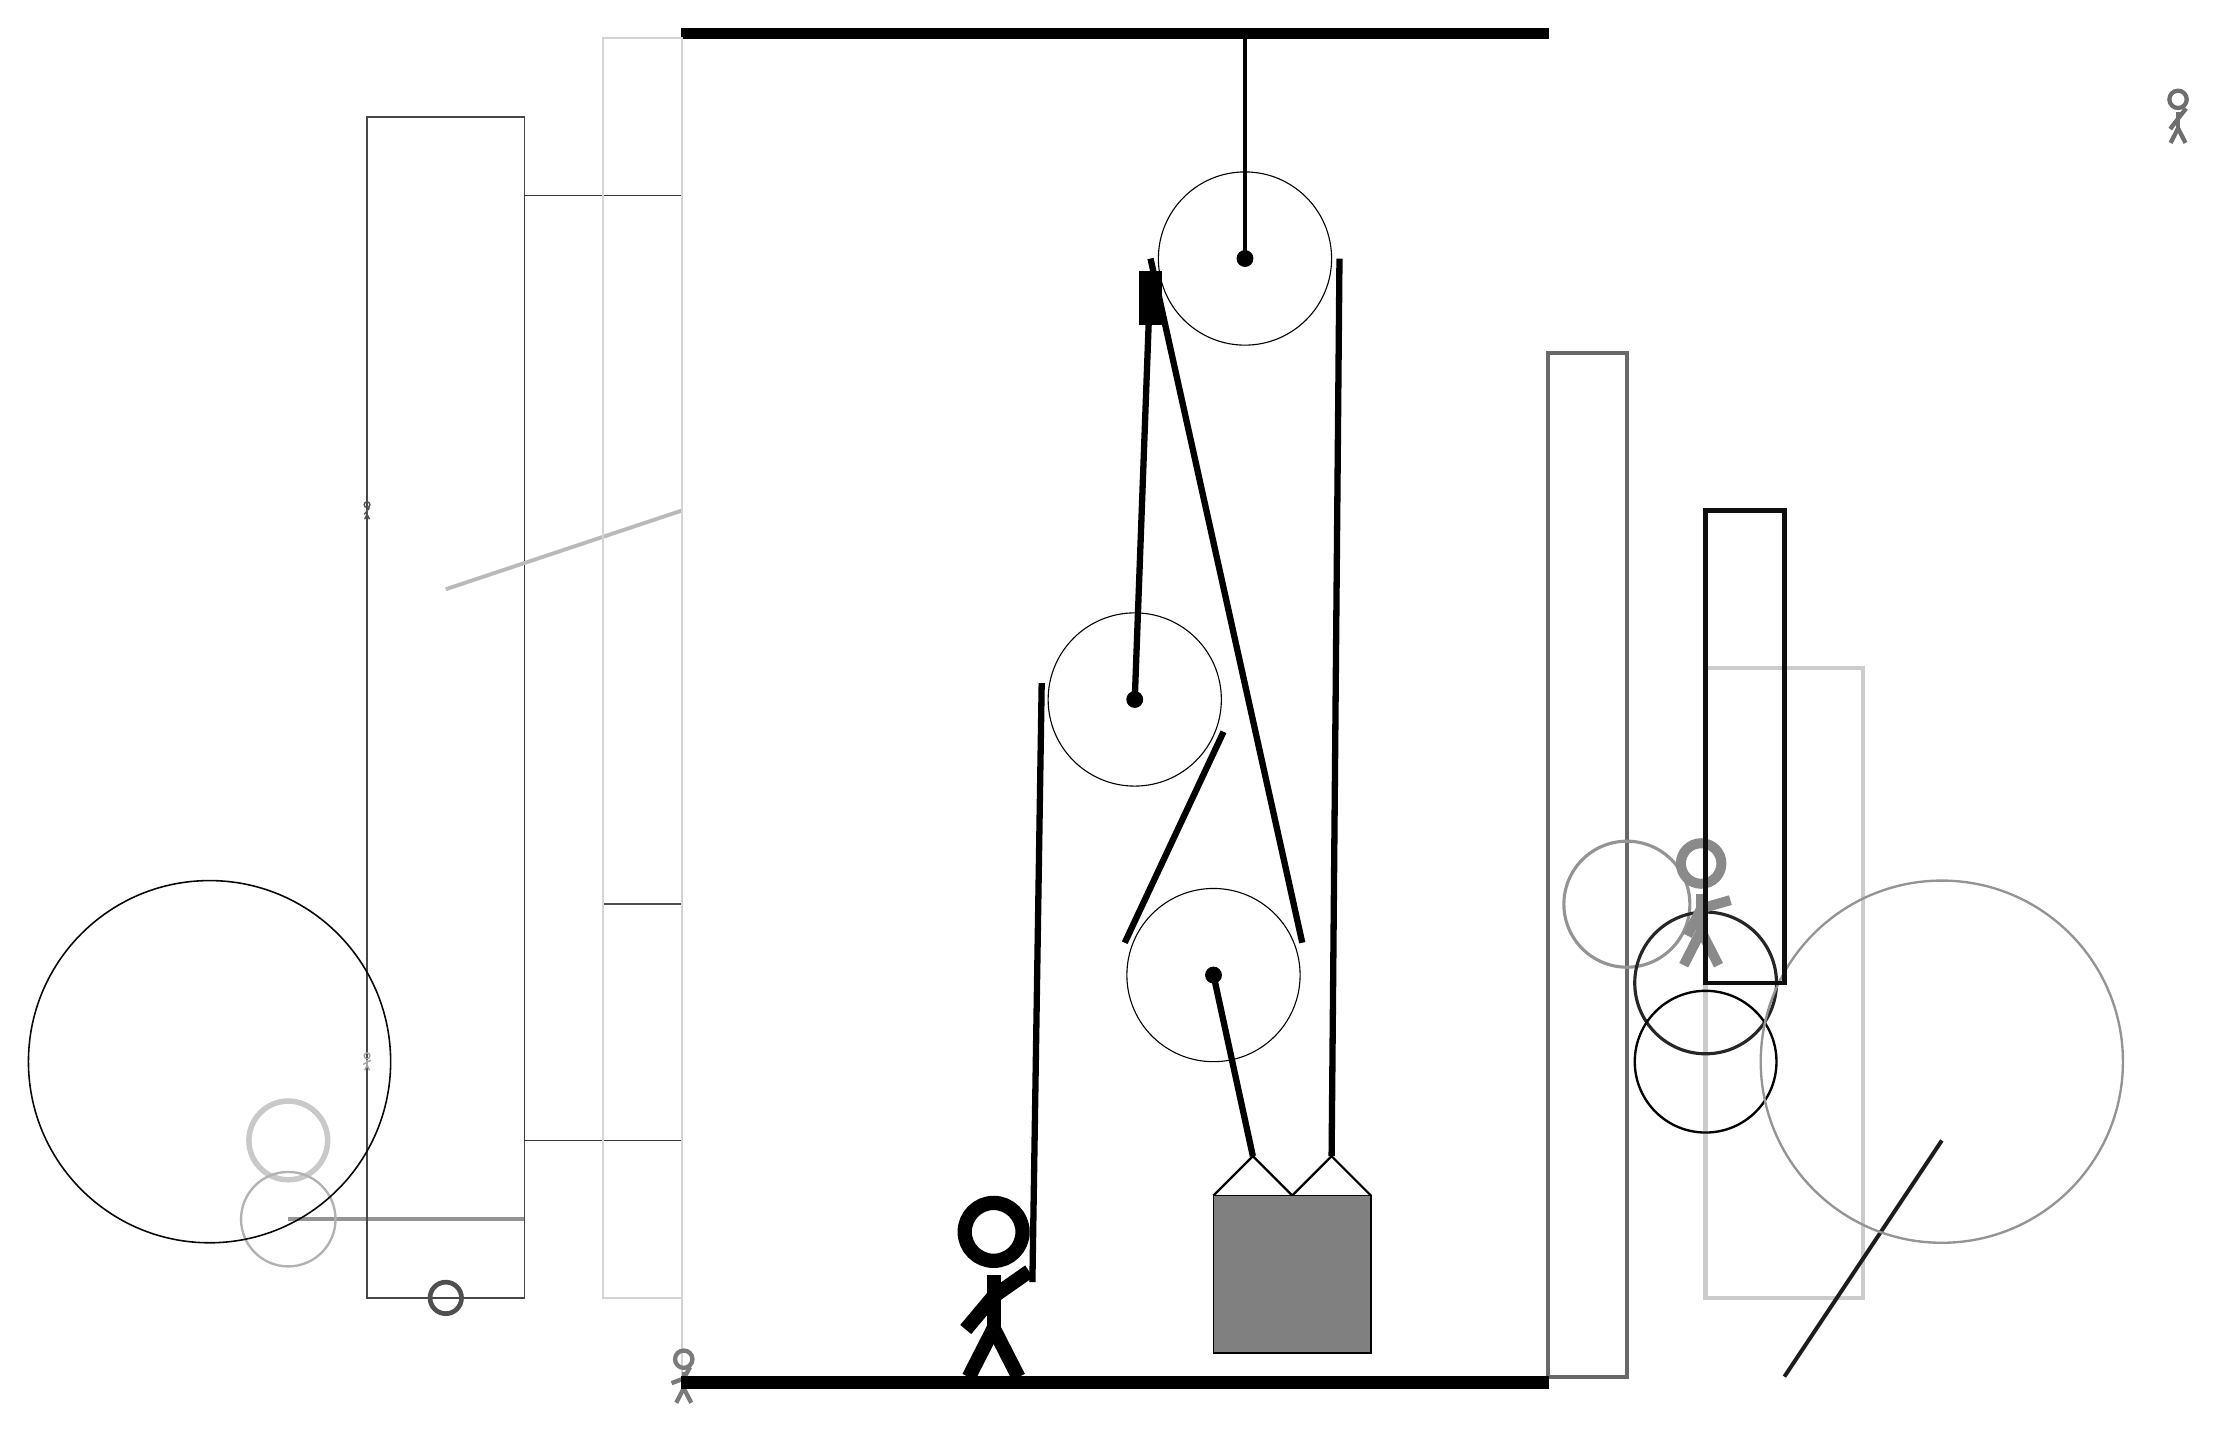
\begin{tikzpicture}
			%%%%% START %%%%%
			
			\draw[fill=black] (-6, 14) rectangle (5, 14.125);
			
			\draw (-0.25, 5.6) circle (1.1);
			\draw[fill=black] (-0.25, 5.6) circle (0.1);
			
			\draw (0.75, 2.1) circle (1.1);
			\draw[fill=black] (0.75, 2.1) circle (0.1);
			
			\draw (1.15, 11.2) circle (1.1);
			\draw[fill=black] (1.15, 11.2) circle (0.1);
			\draw[very thick] (1.15, 11.2) -- (1.15, 14);
			
			\draw[thick]  (0.75, -0.7) -- (1.25, -0.2) -- (1.75, -0.7) -- (2.25, -0.2) -- (2.75, -0.7);
			\draw[fill=black!50] (0.75, -0.7) rectangle (2.75, -2.7);
			
			\draw[line width=0.8mm] (-0.25, 5.6) -- (-0.05, 11.0);
			\draw[line width=0.8mm, fill=black](-0.15, 10.4) rectangle (0.05, 11.0);
			\draw[line width=0.8mm] (-1.55, -1.8) -- (-1.4318, 5.8083);
			\centerarc[line width=0.8mm](-0.25, 5.6)(-20:170:1.2000000000000002);
			\draw[line width=0.8mm] (0.8776, 5.1896) -- (-0.3776, 2.5104);
			\centerarc[line width=0.8mm](0.75, 2.1)(160:380:1.2000000000000002);
			\draw[line width=0.8mm] (1.8776, 2.5104) -- (-0.05, 11.2);
			\draw[line width=0.8mm](0.75, 2.1) -- (1.25, -0.2);
			\centerarc[line width=0.8mm](1.15, 11.2)(0:180:1.2000000000000002);
			\draw[line width=0.8mm] (2.35, 11.2) -- (2.25, -0.2);
			
			\node at (-2, -1.9) {\Strichmaxerl[10][50][35]};
			
			\draw[line width=0.5mm, color=black!59] (6, -3) rectangle (5, 10);
			
			\draw [line width=0.4mm, color=black!42](6, 3) circle (0.8);
			\draw[line width=0.2mm, color=black!18] (-6, -3) rectangle (-6, 4);
			\draw[line width=0.5mm, color=black!42](-8, -1) -- (-11, -1);
			\draw[line width=0.6mm, color=black!20] (7, 6) rectangle (9, -2);
			\draw [line width=0.7mm, color=black!21](-11, 0) circle (0.5);
			\draw [line width=0.4mm, color=black!85](7, 2) circle (0.9);
			\draw[line width=0.2mm, color=black!72] (-8, -2) rectangle (-10, 13);
			\draw [line width=0.6mm, color=black!69](-9, -2) circle (0.2);
			\node[line width=0.6mm, color=black!68] at (-10, 8) {\Strichmaxerl[1][49][56]};
			
			\node[line width=0.6mm, color=black!46] at (7, 3) {\Strichmaxerl[7][63][16]};
			\node[line width=0.7mm, color=black!52] at (-6, -3) {\Strichmaxerl[3][21][61]};
			\draw[line width=0.2mm, color=black!78] (-8, 0) rectangle (-6, 12);
			
			\draw [line width=0.3mm, color=black!30](-11, -1) circle (0.6);
			\draw[line width=0.5mm, color=black!89](8, -3) -- (10, 0);
			\draw[line width=0.3mm, color=black!69] (-7, 3) rectangle (-6, -2);
			
			\draw [line width=0.3mm, color=black!99](7, 1) circle (0.9);
			
			\draw [line width=0.3mm, color=black!42](10, 1) circle (2.3);
			\draw [line width=0.2mm, color=black!97](-12, 1) circle (2.3);
			
			\draw[line width=0.6mm, color=black!94] (7, 2) rectangle (8, 8);
			\draw[line width=0.5mm, color=black!27](-6, 8) -- (-9, 7);
			\node[line width=0.5mm, color=black!57] at (13, 13) {\Strichmaxerl[3][53][52]};
			\draw[line width=0.3mm, color=black!17] (-6, -2) rectangle (-7, 14);
			\node[line width=0.2mm, color=black!36] at (-10, 1) {\Strichmaxerl[1][28][30]};
			
			\draw[fill=black] (-6, -3) rectangle (5, -3.15);
			
			%%%%% END %%%%%
		\end{tikzpicture}
	\end{figure}	
\end{document}